\documentclass[12pt,letterpaper]{article}\usepackage[]{graphicx}\usepackage[]{color}
%% maxwidth is the original width if it is less than linewidth
%% otherwise use linewidth (to make sure the graphics do not exceed the margin)
\makeatletter
\def\maxwidth{ %
  \ifdim\Gin@nat@width>\linewidth
    \linewidth
  \else
    \Gin@nat@width
  \fi
}
\makeatother

\definecolor{fgcolor}{rgb}{0.345, 0.345, 0.345}
\newcommand{\hlnum}[1]{\textcolor[rgb]{0.686,0.059,0.569}{#1}}%
\newcommand{\hlstr}[1]{\textcolor[rgb]{0.192,0.494,0.8}{#1}}%
\newcommand{\hlcom}[1]{\textcolor[rgb]{0.678,0.584,0.686}{\textit{#1}}}%
\newcommand{\hlopt}[1]{\textcolor[rgb]{0,0,0}{#1}}%
\newcommand{\hlstd}[1]{\textcolor[rgb]{0.345,0.345,0.345}{#1}}%
\newcommand{\hlkwa}[1]{\textcolor[rgb]{0.161,0.373,0.58}{\textbf{#1}}}%
\newcommand{\hlkwb}[1]{\textcolor[rgb]{0.69,0.353,0.396}{#1}}%
\newcommand{\hlkwc}[1]{\textcolor[rgb]{0.333,0.667,0.333}{#1}}%
\newcommand{\hlkwd}[1]{\textcolor[rgb]{0.737,0.353,0.396}{\textbf{#1}}}%

\usepackage{framed}
\makeatletter
\newenvironment{kframe}{%
 \def\at@end@of@kframe{}%
 \ifinner\ifhmode%
  \def\at@end@of@kframe{\end{minipage}}%
  \begin{minipage}{\columnwidth}%
 \fi\fi%
 \def\FrameCommand##1{\hskip\@totalleftmargin \hskip-\fboxsep
 \colorbox{shadecolor}{##1}\hskip-\fboxsep
     % There is no \\@totalrightmargin, so:
     \hskip-\linewidth \hskip-\@totalleftmargin \hskip\columnwidth}%
 \MakeFramed {\advance\hsize-\width
   \@totalleftmargin\z@ \linewidth\hsize
   \@setminipage}}%
 {\par\unskip\endMakeFramed%
 \at@end@of@kframe}
\makeatother

\definecolor{shadecolor}{rgb}{.97, .97, .97}
\definecolor{messagecolor}{rgb}{0, 0, 0}
\definecolor{warningcolor}{rgb}{1, 0, 1}
\definecolor{errorcolor}{rgb}{1, 0, 0}
\newenvironment{knitrout}{}{} % an empty environment to be redefined in TeX

\usepackage{alltt}
 \usepackage[left=2cm,right=2cm,top=2cm,bottom=2cm]{geometry}
\usepackage[ansinew]{inputenc}
\usepackage[spanish]{babel}
\usepackage{amsmath}
\usepackage{amsfonts}
\usepackage{amssymb}
\usepackage{dsfont}
\usepackage{multicol} 
\usepackage{subfigure}
\usepackage{graphicx}
\usepackage{float} 
\usepackage{verbatim} 
\usepackage[left=2cm,right=2cm,top=2cm,bottom=2cm]{geometry}
\usepackage{fancyhdr}
\pagestyle{fancy} 
\fancyhead[LO]{\leftmark}
\usepackage{caption}
\newtheorem{definicion}{Definci\'on}
\IfFileExists{upquote.sty}{\usepackage{upquote}}{}
\begin{document}

\begin{titlepage}
\setlength{\unitlength}{1 cm} %Especificar unidad de trabajo


\begin{center}
\textbf{{\large UNIVERSIDAD DE EL SALVADOR}\\ [0.50 cm]
{\large FACULTAD MULTIDISCIPLINARIA DE OCCIDENTE}\\ [0.50 cm]
{\large DEPARTAMENTO DE MATEM\'ATICA}}\\[0.50 cm]

\begin{picture}(18,4)
 \put(7,0){
\includegraphics[width=4cm]{minerva.jpg}}
\end{picture}
\\[0.25 cm]

\textbf{{\large Licenciatura en Estad\'istica}\\[1.25cm]
{\large Control Estadistico del Paquete R }\\[2 cm]
%\setlength{\unitlength}{1 cm}
{\large  \textbf{''UNIDAD CUATRO"}}\\[2cm]
{\large Alumna:}\\
{\large Erika Beatr\'iz Guill\'en Pineda}\\[2cm]
{\large Fecha de elaboraci\'on}\\
Santa Ana - \today }
\end{center}
\end{titlepage}

\newtheorem{teorema}{Teorema}
\newtheorem{prop}{Proposici\'on}[section]

\lhead{PR\'ACTICA 17}
\lfoot{LICENCIATURA EN ESTAD\'ISTICA}
\cfoot{UESOCC}
\rfoot{\thepage}
%\pagestyle{fancy} 

\setcounter{page}{1}
\newpage


\section{INTRODUCCI\'ON}

La Inferencia Estad\'istica es: El conjunto de m\'etodos estad\'isticos que permiten deducir (inferir) como se distribuye (comporta) la poblaci\'on en estudio o las relaciones estoc\'asticas entre varias variables de inter\'es a partir de la informaci\'on suministrada por una muestra aleatoria.\\

La Inferencia Estad\'istica param\'etrica plantea tres tipos de problemas:
\begin{itemize}
  \item Estimaci\'on puntual: en la que pretendemos dar un valor puntual del par\'ametro. 
  \item Estimaci\'on por intervalos: en elque buscamos un intervalo en el que confiamos se encuentre el verdadero valor de teta desconocido.
  \item Contraste de hip\'otesis: donde buscamos probar una declaraci\'on o un supuesto acerca del valor de uno (o m\'as) par\'ametro(s) teta. 
\end{itemize}

Para llevar a cabo lo anterior, se parte del supuesto de que la distribuci\'on de la(s) caracter\'istica(s) que se est\'a estudiando pertenece a una familia conocida de distribuciones, siendo \'unicamente desconocidos los par\'ametros que la definen. Por lo regular pertenecen a la familia normal o a cualquiera que pueda obtenerse a partir de ella como lo es: la t de Student, la Chi-Cuadrado o la F de Snedecor.

\section{ESTIMACI\'ON PUNTUAL}\\[1cm]

Un estad\'istico teta estimado es igual a f($X_1$, $X_2$, $X_3$,...,$X_n$) es un estimador adecuado de un par\'ametro teta, si cumple las siguientes propiedades: 
\begin{itemize}
  \item \textbf{Insesgadez:}
  si la esperanza matem\'atica del estimador coincide con el valor del par\'ametro al cual 
est\'a intentado estimar E[teta estimado]=teta. Es decir, la distribuci\'on de probabilidad del estimador se concentra alrededor del valor que intenta predecir.
\item \textbf{Consistencia:}
si el estimador converge en probabilidad al valor del par\'ametro que est\'a 
intentado estimar conforme crece el tama\~no de la muestra. Es decir si $\~teta_n$ representa el estimador para una muestra de tama\~no n, entonces se dice que $\~teta$ es consistente si: 
el limite de n cuando tiende a infinito de E[teta estimado]=teta.
\item \textbf{Eficiencia:}
si entre todos los posibles estimadores (insesgados o no) que pueden obtenerse es el que tenga la menor varianza posible.
\end{itemize}\\[1cm]

\textbf{Se verifica f\'acilmente que la media muestral (estimador de la media poblacional) cumple estas tres y a\'un m\'as propiedades.}\\[1cm]


\section{ESTIMACI\'ON POR INTERVALOS DE CONFIANZA.}


La idea de la estimaci\'on por intervalos de confianza radica en encontrar dos n\'umeros reales, digamos $\~teta_1$ y $\~teta_2$, tales que el par\'ametro desconocido $teta$ que se quiere estimar pertenezca al intervalo formado por dichos valores con probabilidad alta, digamos $1-a$.  Es decir;
\begin{center}
P[$\~teta_1$$<$=$teta$$<$=$\~teta_2$]=$1-a$
\end{center}
Donde $\~teta_1$ y $\~teta_2$ sean valores  que dependan \'unicamente del estimador $\~teta$ y de los valores observados en la muestra $X_1$, $X_2$, $X_3$,...,$X_n$.\\

Se verifica f\'acilmente que cuando la caracter\'istica de inter\'es X sigue una distribuci\'on conocida la cual es sim\'etrica (como la normal o la binomial o sus derivadas), y adem\'as los estimadores son insesgados los mejores intervalos, en el sentido de su anchura, son los intervalos sim\'etricos alrededor del par\'ametro a estimar.\\

Hay que tener en cuenta que $1-a$: es la probabilidad de que par\'ametro se encuentre en el intervalo antes de extraer la muestra. Una vez seleccionada la muestra esta probabilidad es 1 \'o 0, dependiendo de si el par\'ametro se encuentra o no en el intervalo. En este sentido es que no se habla de probabilidad sino de confianza.\\

El concepto de confianza puede interpretarse de la siguiente manera: si se repitiera el experimento muestral (se tomar\'an muchas muestras) muchas veces, en aproximadamente el $100($1-a$)\%$ de los casos se confiar\'ia que los intervalos de confianza encontrados contengan al verdadero valor del par\'ametro $teta$ a estimar.

\section{SIMULACI\'ON DEL CONCEPTO DE INTERVALO DE CONFIANZA PARA ESTIMAR UN PAR\'AMETRO.}


\begin{itemize}
  \item \tetxtbf{Ejemplo 1:}
\end{itemize}
Sea la variable aleatoria X = el n\'umero de caras obtenidas, al lanzar una moneda balanceada 20 veces. Simulamos 50 muestras para generar intervalos de 95\% de confianza y as\'i poder estimar la proporci\'on verdadera de caras (p), y encontrar en cu\'antos de estos intervalos se encuentra el verdadero valor de la proporci\'on.\\

Entonces X tiene una distribuci\'on binomial con p\'arametros n=20 y p=0.5.\\

La funci\'on para generar cada una de las muestras, junto con los l\'imites inferior y superior de los intervalos de confianza se muestra en seguida y le hemos llamado "simulIntProp". 
\begin{knitrout}
\definecolor{shadecolor}{rgb}{0.969, 0.969, 0.969}\color{fgcolor}\begin{kframe}
\begin{alltt}
\hlstd{simulIntProp} \hlkwb{<-} \hlkwa{function}\hlstd{(}\hlkwc{m}\hlstd{=}\hlnum{5}\hlstd{,} \hlkwc{n}\hlstd{=}\hlnum{1}\hlstd{,} \hlkwc{p}\hlstd{,} \hlkwc{nivel.conf}\hlstd{=}\hlnum{0.95}\hlstd{)}
\hlstd{\{}
\hlstd{X} \hlkwb{<-} \hlkwd{rbinom}\hlstd{(m, n, p)}
\hlcom{# Matriz con 1000 valores aleatorios binomial(n,p), 50 muestras cada una de tamaño 20 }
\hlstd{pe} \hlkwb{<<-} \hlstd{X}\hlopt{/}\hlstd{n}
 \hlcom{# Calcula la proporción estimada en cada una de las muestras. }
\hlstd{SE} \hlkwb{<<-} \hlkwd{sqrt}\hlstd{(pe}\hlopt{*}\hlstd{(}\hlnum{1}\hlopt{-}\hlstd{pe)}\hlopt{/}\hlstd{n)}
\hlcom{# Calcula la desviación estándar estimada en cada una de las muestras. }
\hlstd{alfa} \hlkwb{<-} \hlnum{1}\hlopt{-}\hlstd{nivel.conf}
\hlstd{z} \hlkwb{<<-} \hlkwd{qnorm}\hlstd{(}\hlnum{1}\hlopt{-}\hlstd{alfa}\hlopt{/}\hlnum{2}\hlstd{)}
\hlstd{Intervalo} \hlkwb{<<-} \hlkwd{cbind}\hlstd{(pe} \hlopt{-} \hlstd{z}\hlopt{*}\hlstd{SE, pe} \hlopt{+} \hlstd{z}\hlopt{*}\hlstd{SE)}
\hlcom{# genera los extremos del intervalo de confianza }
\hlstd{nInter} \hlkwb{<<-} \hlnum{0}
\hlcom{# un contador para conocer en cuántos intervalos se encuentra la verdadera proporción. }
\hlkwa{for}\hlstd{(i} \hlkwa{in} \hlnum{1}\hlopt{:}\hlstd{m)}
\hlkwa{if} \hlstd{((p} \hlopt{>=} \hlstd{Intervalo[i,} \hlnum{1}\hlstd{])} \hlopt{&&} \hlstd{(p} \hlopt{<=} \hlstd{Intervalo[i,} \hlnum{2}\hlstd{]))}
\hlstd{nInter} \hlkwb{<<-} \hlstd{nInter} \hlopt{+} \hlnum{1}
\hlcom{# función que cuenta cuántos intervalos contienen el verdadero valor del parámetro. }
\hlkwd{return}\hlstd{(nInter)}
\hlstd{\}}
\hlstd{n}\hlkwb{=}\hlnum{20}\hlstd{; m}\hlkwb{=} \hlnum{50}\hlstd{; p}\hlkwb{=}\hlnum{0.5}\hlstd{; nivel.conf}\hlkwb{=}\hlnum{0.95}
\hlkwd{simulIntProp}\hlstd{(m, n, p, nivel.conf)}
\end{alltt}
\begin{verbatim}
## [1] 49
\end{verbatim}
\begin{alltt}
\hlstd{Intervalo} \hlcom{# para visualizar cada uno de los intervalos generados }
\end{alltt}
\begin{verbatim}
##             [,1]      [,2]
##  [1,] 0.18529670 0.6147033
##  [2,] 0.23196777 0.6680322
##  [3,] 0.33196777 0.7680322
##  [4,] 0.38529670 0.8147033
##  [5,] 0.23196777 0.6680322
##  [6,] 0.56022730 0.9397727
##  [7,] 0.18529670 0.6147033
##  [8,] 0.14096270 0.5590373
##  [9,] 0.38529670 0.8147033
## [10,] 0.14096270 0.5590373
## [11,] 0.28086936 0.7191306
## [12,] 0.33196777 0.7680322
## [13,] 0.18529670 0.6147033
## [14,] 0.38529670 0.8147033
## [15,] 0.23196777 0.6680322
## [16,] 0.14096270 0.5590373
## [17,] 0.14096270 0.5590373
## [18,] 0.23196777 0.6680322
## [19,] 0.44096270 0.8590373
## [20,] 0.44096270 0.8590373
## [21,] 0.09916346 0.5008365
## [22,] 0.38529670 0.8147033
## [23,] 0.23196777 0.6680322
## [24,] 0.38529670 0.8147033
## [25,] 0.38529670 0.8147033
## [26,] 0.44096270 0.8590373
## [27,] 0.38529670 0.8147033
## [28,] 0.18529670 0.6147033
## [29,] 0.33196777 0.7680322
## [30,] 0.44096270 0.8590373
## [31,] 0.14096270 0.5590373
## [32,] 0.28086936 0.7191306
## [33,] 0.18529670 0.6147033
## [34,] 0.28086936 0.7191306
## [35,] 0.49916346 0.9008365
## [36,] 0.28086936 0.7191306
## [37,] 0.18529670 0.6147033
## [38,] 0.33196777 0.7680322
## [39,] 0.23196777 0.6680322
## [40,] 0.14096270 0.5590373
## [41,] 0.23196777 0.6680322
## [42,] 0.44096270 0.8590373
## [43,] 0.44096270 0.8590373
## [44,] 0.28086936 0.7191306
## [45,] 0.23196777 0.6680322
## [46,] 0.23196777 0.6680322
## [47,] 0.38529670 0.8147033
## [48,] 0.23196777 0.6680322
## [49,] 0.33196777 0.7680322
## [50,] 0.38529670 0.8147033
\end{verbatim}
\begin{alltt}
\hlstd{nInter} \hlcom{# para visualizar en cuántos de estos intervalos se encuentra la }
\end{alltt}
\begin{verbatim}
## [1] 49
\end{verbatim}
\begin{alltt}
\hlcom{# verdadera proporción.}
\end{alltt}
\end{kframe}
\end{knitrout}

Gr\'afico que muestra los intervalos de confianza de 95\% que contienen y no contienen el verdadero valor del par\'ametro p. 
\begin{knitrout}
\definecolor{shadecolor}{rgb}{0.969, 0.969, 0.969}\color{fgcolor}\begin{kframe}
\begin{alltt}
\hlkwd{matplot}\hlstd{(}\hlkwd{rbind}\hlstd{(pe} \hlopt{-} \hlstd{z}\hlopt{*}\hlstd{SE, pe} \hlopt{+} \hlstd{z}\hlopt{*}\hlstd{SE),} \hlkwd{rbind}\hlstd{(}\hlnum{1}\hlopt{:}\hlstd{m,} \hlnum{1}\hlopt{:}\hlstd{m),} \hlkwc{type}\hlstd{=}\hlstr{"l"}\hlstd{,} \hlkwc{lty}\hlstd{=}\hlnum{1}\hlstd{)}
\hlkwd{abline}\hlstd{(}\hlkwc{v}\hlstd{=p)}
\end{alltt}
\end{kframe}
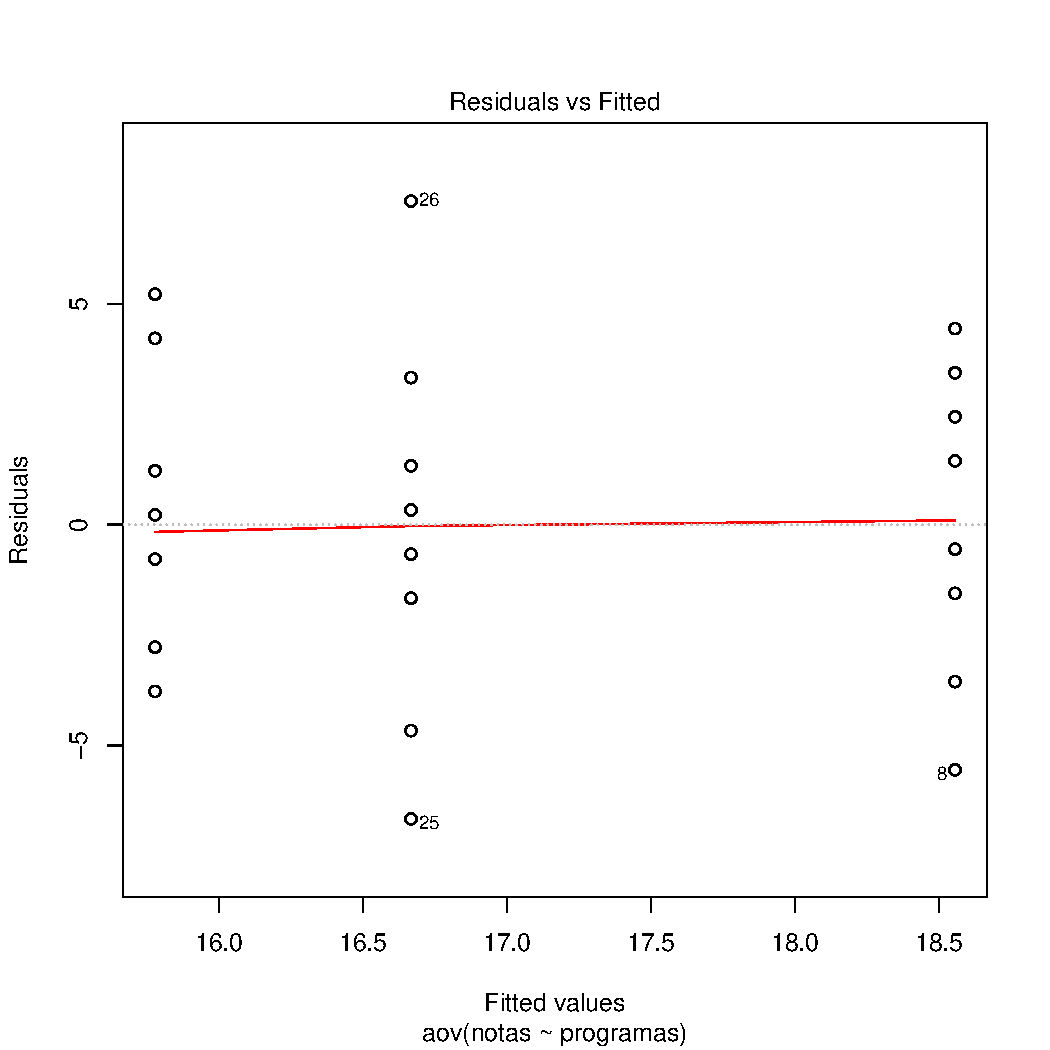
\includegraphics[width=\maxwidth]{figure/unnamed-chunk-2-1} 

\end{knitrout}
\newpage
\begin{itemize}
  \item \textbf{Ejercicio 1:}
\end{itemize}
Sea la variable aleatoria X = el n\'umero que se obtiene al lanzar un dado no cargado 30 veces. Simular 56 muestras para generar intervalos de 95\% de confianza para estimar el promedio $(\µ)$, y encontrar cu\'antos de estos intervalos contiene el valor medio verdadero.
\begin{knitrout}
\definecolor{shadecolor}{rgb}{0.969, 0.969, 0.969}\color{fgcolor}\begin{kframe}
\begin{alltt}
\hlstd{simulIntProp} \hlkwb{<-} \hlkwa{function}\hlstd{(}\hlkwc{m}\hlstd{=}\hlnum{5}\hlstd{,} \hlkwc{n}\hlstd{=}\hlnum{1}\hlstd{,} \hlkwc{p}\hlstd{,} \hlkwc{nivel.conf}\hlstd{=}\hlnum{0.95}\hlstd{)}
\hlstd{\{}
\hlstd{X} \hlkwb{<-} \hlkwd{rbinom}\hlstd{(m, n, p)}
\hlcom{# Matriz con 1000 valores aleatorios binomial(n,p), 56 muestras cada una de tamaño 30 }
\hlstd{pe} \hlkwb{<<-} \hlstd{X}\hlopt{/}\hlstd{n}
 \hlcom{# Calcula la proporción estimada en cada una de las muestras. }
\hlstd{SE} \hlkwb{<<-} \hlkwd{sqrt}\hlstd{(pe}\hlopt{*}\hlstd{(}\hlnum{1}\hlopt{-}\hlstd{pe)}\hlopt{/}\hlstd{n)}
\hlcom{# Calcula la desviación estándarestimada en cada una de las muestras. }
\hlstd{alfa} \hlkwb{<-} \hlnum{1}\hlopt{-}\hlstd{nivel.conf}
\hlstd{z} \hlkwb{<<-} \hlkwd{qnorm}\hlstd{(}\hlnum{1}\hlopt{-}\hlstd{alfa}\hlopt{/}\hlnum{2}\hlstd{)}
\hlstd{Intervalo} \hlkwb{<<-} \hlkwd{cbind}\hlstd{(pe} \hlopt{-} \hlstd{z}\hlopt{*}\hlstd{SE, pe} \hlopt{+} \hlstd{z}\hlopt{*}\hlstd{SE)}
\hlcom{# genera los extremos del intervalo de confianza }
\hlstd{nInter} \hlkwb{<<-} \hlnum{0}
\hlcom{# un contador para conocer en cuántos intervalos se encuentra la }
\hlcom{#verdadera proporción. }
\hlkwa{for}\hlstd{(i} \hlkwa{in} \hlnum{1}\hlopt{:}\hlstd{m)}
\hlkwa{if} \hlstd{((p} \hlopt{>=} \hlstd{Intervalo[i,} \hlnum{1}\hlstd{])} \hlopt{&&} \hlstd{(p} \hlopt{<=} \hlstd{Intervalo[i,} \hlnum{2}\hlstd{]))}
\hlstd{nInter} \hlkwb{<<-} \hlstd{nInter} \hlopt{+} \hlnum{1}
\hlcom{# función que cuenta cuántos intervalos contienen el verdadero valor del parámetro. }
\hlkwd{return}\hlstd{(nInter)}
\hlstd{\}}
\hlstd{n}\hlkwb{=}\hlnum{30}\hlstd{; m}\hlkwb{=} \hlnum{56}\hlstd{; p}\hlkwb{=}\hlnum{0.17}\hlstd{; nivel.conf}\hlkwb{=}\hlnum{0.95}
\hlkwd{simulIntProp}\hlstd{(m, n, p, nivel.conf)}
\end{alltt}
\begin{verbatim}
## [1] 54
\end{verbatim}
\begin{alltt}
\hlstd{Intervalo} \hlcom{# para visualizar cada uno de los intervalos generados }
\end{alltt}
\begin{verbatim}
##               [,1]       [,2]
##  [1,]  0.033308009 0.30002532
##  [2,] -0.007351649 0.20735165
##  [3,]  0.081984476 0.38468219
##  [4,]  0.011691522 0.25497514
##  [5,]  0.033308009 0.30002532
##  [6,]  0.108424383 0.42490895
##  [7,]  0.011691522 0.25497514
##  [8,] -0.030900702 0.09756737
##  [9,]  0.011691522 0.25497514
## [10,] -0.007351649 0.20735165
## [11,]  0.011691522 0.25497514
## [12,]  0.011691522 0.25497514
## [13,]  0.056864469 0.34313553
## [14,] -0.007351649 0.20735165
## [15,]  0.081984476 0.38468219
## [16,]  0.136017648 0.46398235
## [17,]  0.164646492 0.50202017
## [18,]  0.011691522 0.25497514
## [19,]  0.056864469 0.34313553
## [20,]  0.033308009 0.30002532
## [21,]  0.164646492 0.50202017
## [22,]  0.011691522 0.25497514
## [23,]  0.011691522 0.25497514
## [24,]  0.056864469 0.34313553
## [25,] -0.022594020 0.15592735
## [26,]  0.011691522 0.25497514
## [27,] -0.007351649 0.20735165
## [28,] -0.007351649 0.20735165
## [29,] -0.007351649 0.20735165
## [30,]  0.011691522 0.25497514
## [31,]  0.033308009 0.30002532
## [32,]  0.011691522 0.25497514
## [33,]  0.056864469 0.34313553
## [34,]  0.033308009 0.30002532
## [35,]  0.033308009 0.30002532
## [36,]  0.081984476 0.38468219
## [37,]  0.033308009 0.30002532
## [38,]  0.056864469 0.34313553
## [39,] -0.007351649 0.20735165
## [40,] -0.007351649 0.20735165
## [41,]  0.056864469 0.34313553
## [42,] -0.007351649 0.20735165
## [43,]  0.011691522 0.25497514
## [44,]  0.108424383 0.42490895
## [45,]  0.011691522 0.25497514
## [46,]  0.011691522 0.25497514
## [47,] -0.007351649 0.20735165
## [48,]  0.011691522 0.25497514
## [49,]  0.081984476 0.38468219
## [50,]  0.011691522 0.25497514
## [51,]  0.011691522 0.25497514
## [52,]  0.011691522 0.25497514
## [53,]  0.081984476 0.38468219
## [54,]  0.081984476 0.38468219
## [55,] -0.007351649 0.20735165
## [56,]  0.033308009 0.30002532
\end{verbatim}
\begin{alltt}
\hlstd{nInter} \hlcom{# para visualizar en cuántos de estos intervalos se encuentra la }
\end{alltt}
\begin{verbatim}
## [1] 54
\end{verbatim}
\begin{alltt}
\hlcom{# verdadero valor medio.}
\end{alltt}
\end{kframe}
\end{knitrout}




\end{document}
